\cotefile{71}
\scanpage{3}

\diagram{\resizebox{\linewidth}{!}{{\small\setlength{\arraycolsep}{3pt}
$\begin{array}{ccc|l@{\quad}l}
V_1&V_2&V_3&V_1\ \text{\unsure{borde|bordes}}\ \Gamma'_2,\Gamma'_3&
\Gamma'_1\ \text{\unsure{bordé} par}\ V_2,V_3\\
\overset{\deleted{\unsure{\circ|\bullet}}}{\Gamma}''_1&
\overset{\deleted{\circ}}{\Gamma}''_2&
\overset{\deleted{\circ}}{\Gamma}''_3&
V_2\ \text{borde}\ \Gamma'_3,\Gamma'_1&\Gamma'_2\ \text{---}\ V_3,V_1\\
\shortparallel&\shortparallel&\shortparallel&&\\[-.4ex]
\Gamma'_1-\unsure{\partial|\delta}&\Gamma'_2-\partial&\Gamma'_3-\partial&
V_3\ \text{borde}\ \Gamma'_1,\Gamma'_2&\Gamma'_3\ \text{---}\ V_1,V_2
\end{array}$}}}

\[
\partial=\{\unsure{x},y\}
\]

\[
\begin{aligned}
\Gamma_1&=\Gamma_2\cup\Gamma_3=\Gamma'_{\unsure{2|1}}\cup\Gamma'_3
=\Gamma''_1\cup\Gamma''_2\cup\partial\\
\Gamma_2&=\Gamma_3\cup\Gamma_1=\Gamma'_3\cup\Gamma'_1
=\Gamma''_3\cup\Gamma''_1\cup\unsure{\dot\partial|\partial}\\
\Gamma_3&=\Gamma_1\cup\Gamma_2=\Gamma'_1\cup\Gamma'_2
=\Gamma''_1\cup\Gamma''_2\cup\partial
\end{aligned}
\]

\noindent\begin{minipage}[c]{.34\linewidth}
% The lettering in the drawing is turned a quarter turn on the sheet.
\figure{\resizebox{\linewidth}{!}{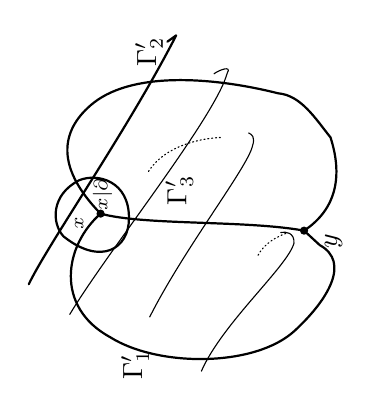
\begin{tikzpicture}[x=.8cm,y=.8cm,line cap=round,line join=round]
\begin{scope}[rotate=90]
\draw[thick] (0,1.25) .. controls (-.51,1.83) and (-1.48,1.98) .. (-1.96,1.10)
 .. controls (-2.44,.34) and (-2.44,-1.20) .. (-1.86,-1.83)
 .. controls (-1.37,-2.36) and (-.77,-2.72) .. (-.50,-2.23) -- (-.27,-1.98);
\draw[thick] (0,1.25) .. controls (.79,2.02) and (1.37,1.85) .. (1.76,1.36)
 .. controls (2.29,.68) and (2.14,-.66) .. (1.91,-1.57)
 .. controls (1.88,-1.93) and (1.51,-2.16) .. (1.21,-2.40)
 .. controls (.62,-2.59) and (.08,-2.51) .. (-.27,-1.98);
\draw[thick] (0,1.25) .. controls (-.19,.56) and (-.10,-1.05) .. (-.27,-1.98);
\draw[thick] (-.36,1.84) .. controls (-.84,1.24) and (-.55,.80) .. (-.08,.80)
 .. controls (.52,.79) and (.65,1.30) .. (.53,1.59) .. controls (.30,2.04) and (-.15,2.03) .. cycle;
\draw[thick] (-1.12,2.39) .. controls (-.49,2.09) and (1.36,.80) .. (2.83,.05) -- (2.73,.19);
\draw (-1.60,1.74) .. controls (-.60,1.14) and (1.53,-.57) .. (2.23,-.76) .. controls (2.36,-.84) and (2.28,-.63) .. (2.22,-.55);
\draw (-1.64,.47) .. controls (-.55,-.08) and (.73,-1.08) .. (1.07,-1.16) .. controls (1.22,-1.21) and (1.26,-1.15) .. (1.28,-1.10);
\draw (-2.50,-.35) .. controls (-1.73,-.69) and (-.85,-1.71) .. (-.47,-1.82) .. controls (-.30,-1.83) and (-.28,-1.69) .. (-.30,-1.61);
\draw[densely dotted] (.67,.49) .. controls (1.09,.22) and (1.20,-.36) .. (1.21,-.68);
\draw[densely dotted] (-.66,-1.25) .. controls (-.47,-1.35) and (-.36,-1.55) .. (-.30,-1.73);
\fill (0,1.25) circle (.065); \fill (-.27,-1.98) circle (.065);
\node[rotate=90] at (-2.40,.70) {$\Gamma'_1$};
\node[rotate=90] at (2.57,.48) {$\Gamma'_{\unsure{2}}$};
\node[rotate=90] at (.37,.00) {$\Gamma'_3$};
\node[rotate=90,inner sep=0pt] at (-.16,1.59) {\scriptsize $\unsure{x}$};
\node[rotate=90,inner sep=0pt] at (.31,1.22) {\scriptsize $\deleted{\unsure{x|\partial}}$};
\node[rotate=90] at (-.44,-2.45) {$y$};
\end{scope}
\end{tikzpicture}}}
\end{minipage}\hfill
\begin{minipage}[c]{.64\linewidth}
\[
\resizebox{\linewidth}{!}{$\displaystyle
\Gamma_3^{\deleted{\unsure{\circ|'}}}=\Gamma''_1\cup\Gamma''_{\unsure{2|1}}\cup\partial
\ \big|\quad U_3=V_1\cup V_2\cup\Gamma''_3\quad\big|\quad V_3$}
\]

\[
\dot U_3=\Gamma_3\qquad U_3\cup
\]
\end{minipage}

\[
\unsure{\cdot}\ U,C,V
\]
% archive sheet number: 2
\scanpage{4}
\begingroup\ttfamily

% letterhead
\noindent
\begin{minipage}[t]{.48\linewidth}\centering
U N I V E R S I T E\\
DES SCIENCES ET TECHNIQUES\\
DU LANGUEDOC\\
{\footnotesize $\frown\frown\frown\frown\frown\frown\frown\frown\frown\frown\frown\frown$}\\[.6em]
Service de la Scolarité\\
JP/GJ\\[.5em]
\uline{Diffusion} : Liste A\\
N°: 2418
\end{minipage}\hfill
\begin{minipage}[t]{.49\linewidth}\raggedleft
MONTPELLIER, le 19 AVRIL 1977\\
\end{minipage}

\begin{center}
\uline{AVIS DE SOUTENANCE D'UNE THESE DE DOCTORAT DE}\\[.5em]
\uline{SPECIALITE : SCIENCES DE LA TERRE mention GEOLOGIE APPLIQUEE}
\end{center}

\uline{Nom et prénom du candidat} : BAYER Michel

\uline{Titre de la thèse} : Etude gravimétrique de la Corse.

\uline{Date, heure et lieu de soutenance prévus} : 25 AVRIL 1977 à 14 h. 30

\hspace*{3em}Salle de cours n° 10 - U.S.T.L.

\uline{Nom du Directeur de thèse} : M. LOUIS Pierre

\uline{Désignation du laboratoire où la thèse est préparée} :

\hspace*{3em}Laboratoire de Géophysique

\uline{Analyse de l'ouvrage} : Afin de terminer le levé gravimétrique de la Corse, 270 mesures ont été effectuées. L'ensemble des données (720 stations) a été traité (cartes de l'anomalie de Bouguer, dérivées, régionales et résiduelles) puis interprété, en tenant compte de la géologie et de l'aéromagnétisme. Des hypothèses sont proposées, en particulier pour la structure profonde de la Corse et des régions avoisinantes (bassin Algéro-provençal).

\uline{Durée approximative des recherches ayant abouti à la thèse} : Deux ans

\uline{Composition du jury proposé} :

\begin{center}
\begin{tabular}{r@{\quad}l}
MM. : & P. LOUIS\\
      & M. MATTAUER\\
      & R. NEUMANN\\
Mlle  & F. RIMBERT\\
M.    & J. ORSINI
\end{tabular}
\end{center}

\noindent\hfill\begin{minipage}{.49\linewidth}\centering
Le Secrétaire Général,\\[.7em]
\figure{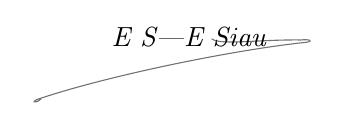
\begin{tikzpicture}[x=.70cm,y=.70cm,line cap=round]
\draw[thin,black!55] (-2.22,-.72) .. controls (-2.32,-.82) and (-2.45,-.77) .. (-2.20,-.70)
 .. controls (-.96,-.29) and (1.27,.17) .. (2.61,.31)
 .. controls (2.72,.33) and (2.66,.37) .. (2.50,.35)
 .. controls (1.70,.36) and (1.04,.25) .. (.88,.37);
\node[anchor=base,inner sep=0pt] at (.46,.23) {\normalfont\itshape\handwritten{\unsure{E S|E Siau}}};
\end{tikzpicture}}
\uline{E. SIAU}\\
\end{minipage}
\endgroup
% archive sheet number: 3
\scanpage{6}

$\unsure{\mathcal{X}|\mathscr{X}}$ qui est \unsure{aussi} la \unsure{somme amalgamée} de\deleted{\unsure{s}} $\overline W$ et de\deleted{s} $\coprod_{i\in I}\overline U_i$ (\unsure{sur}
\diagram{\begin{tikzcd}[ampersand replacement=\&,row sep=small,column sep=large]
\coprod_i B_i \arrow[r,hook] \arrow[dr] \& \overline W\\
\& \coprod_i\overline U_i
\end{tikzcd}}
) :

\noindent\begin{minipage}[c]{.41\linewidth}
\figure{\resizebox{\linewidth}{!}{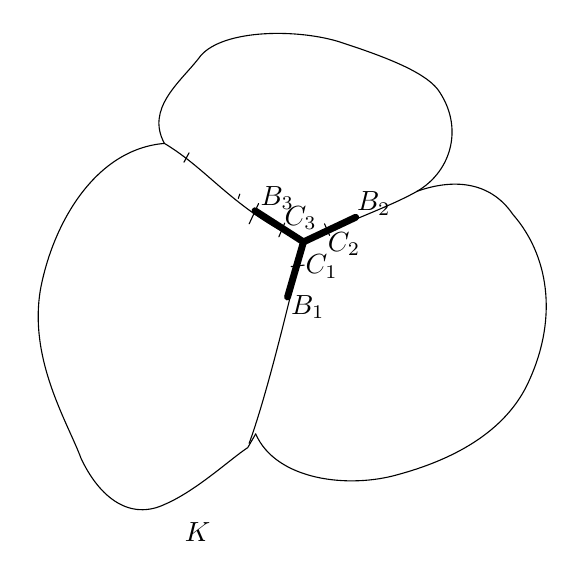
\begin{tikzpicture}[x=.92cm,y=.92cm,line cap=round,line join=round]
\draw (-1.92,1.36) .. controls (-2.18,1.84) and (-1.71,2.20) .. (-1.45,2.53)
 .. controls (-1.18,2.93) and (-.14,2.95) .. (.47,2.77)
 .. controls (1.09,2.57) and (1.65,2.36) .. (1.85,2.11)
 .. controls (2.22,1.60) and (2.05,.98) .. (1.57,.70);
\draw (-1.92,1.36) .. controls (-2.88,1.28) and (-3.46,.25) .. (-3.63,-.65)
 .. controls (-3.80,-1.63) and (-3.25,-2.50) .. (-3.07,-2.99)
 .. controls (-2.81,-3.54) and (-2.39,-3.85) .. (-1.91,-3.62)
 .. controls (-1.47,-3.43) and (-.99,-2.98) .. (-.77,-2.84) -- (-.66,-2.65);
\draw (-.66,-2.65) .. controls (-.38,-3.29) and (.62,-3.41) .. (1.31,-3.21)
 .. controls (2.26,-2.95) and (2.87,-2.50) .. (3.13,-1.88)
 .. controls (3.51,-1.02) and (3.38,-.18) .. (2.89,.38)
 .. controls (2.57,.85) and (2.05,.87) .. (1.57,.70);
\draw (-1.92,1.36) .. controls (-1.30,.99) and (-.96,.44) .. (0,0);
\draw (0,0) .. controls (.67,.31) and (1.20,.49) .. (1.57,.70);
\draw (0,0) .. controls (-.23,-.96) and (-.51,-2.12) .. (-.75,-2.78);
\draw[line width=2.5pt] (-.67,.43) -- (0,0) -- (.72,.34);
\draw[line width=2.5pt] (0,0) -- (-.22,-.76);
\draw (-1.65,1.10)--(-1.58,1.23) (-.90,.60)--(-.88,.66) (-.75,.25)--(-.62,.53)
 (-.34,.07)--(-.26,.26) (.36,.09)--(.29,.25) (-.17,-.34)--(.01,-.32);
\node at (-.36,.60) {$B_3$}; \node at (-.04,.33) {$C_3$};
\node at (.97,.53) {$B_2$}; \node at (.56,-.03) {$C_2$};
\node at (.25,-.34) {$C_1$}; \node at (.06,-.90) {$B_1$};
\node at (-1.46,-4.00) {$K$};
\end{tikzpicture}}}
\end{minipage}\hfill
\begin{minipage}[c]{.56\linewidth}
\deleted{L'application \unsure{naturelle}}

\[
\deleted{\unsure{\text{de}}\quad\mathcal{X}\longrightarrow X}
\]

\[
\resizebox{\linewidth}{!}{$\displaystyle
\begin{aligned}
\mathcal X&\simeq\overline W\amalg_{\left(\coprod_i B_i\right)}
 \left(\deleted{\unsure{\bigcup}}\coprod_i\overline U_i\right)\\
&\simeq\coprod_{i\,(\unsure{W|w})}X_i
\end{aligned}
\qquad
\begin{array}{c}
X_{\unsure{w|i}}\simeq\mathcal X_i\\
\phantom{X_i\simeq{}}\shortparallel\\[-.5ex]
\phantom{X_i\simeq{}}\operatorname{Im}X_i
\end{array}$}
\]
\end{minipage}
\margin{\tikz[baseline=-.2ex]{\draw[->] (.38,.25) to[bend right=12] (0,0);} \unsure{ouvert} de $\mathcal X$}

$\mathcal X\longrightarrow X$ est étale en les \unsure{pts} de $\mathcal X\smallsetminus\coprod_i C_i$, c'est une \unsure{imm} fermée en les pts de $\coprod C_i$

6) Énoncé d'\unsure{invariance} de $\mathcal X$ par rapport au \unsure{remplacement} de $K$ par $K^*\subset K$ ($U_i,U'_i$ par $U_i^*=U_i\cap K^*$, \inserted{$U_i'{}^{\unsure{*|\wedge}}=U'_i\cap K^*$}), \unsure{pourvu} que
% slanted
\margin{\unsure{vérifier} l'énoncé \unsure{précis}\ldots}
\deleted{$\unsure{K'|\dot K'}\subset\bigcup U_i$, et} \inserted{$\dot K^*\subset\bigcup U_i$, et} $\deleted{(K\smallsetminus K')^{\unsure{-}}}\ \forall i$, $C_i\subset\overline{U_i^*}\cap\overline{U_i'{}^*}$ (- il suffit que $\deleted{\unsure{K^*|K'}}$ soit $K'\supset\bigcup C_i$

-- vérifier si dans les \unsure{div.} hypothèses précédentes, il n'y avait pas lieu d'exiger $\bigcup C_i\subset\operatorname{int}K$ i.e. $C_i\cap\dot K=\varnothing\quad\forall i\in I$\ldots
\margin{\tikz{\draw[line width=.3pt] (0,0) .. controls (-.04,.25) and (-.05,.6) .. (0,.9);}}
% vertical pen stroke to the left of the last line
\mspage{\unsure{5}}
% archive sheet number: 5
\scanpage{7}

\diagram{\resizebox{\linewidth}{!}{\begin{tikzpicture}[x=.012cm,y=-.012cm,every node/.style={inner sep=1pt}]
\node[anchor=north west] at (30,60) {\begin{tikzcd}[ampersand replacement=\&,row sep=1pt,column sep=2pt]
\& e\in E\\
\& \cup\\
M(e)\ \subset \& E_0=M(E) \arrow[ddd,"\unsure{\varphi|\phi}"]\\[-.4ex]
\shortparallel \&\\[-.4ex]
M(E_e) \&\\
\& I\quad\text{\unsure{ordonné}}
\end{tikzcd}};
\node[anchor=north west] at (575,77) {$\displaystyle
\left\{\begin{aligned}
|E|&=X\supset|E_e|\\
X_i&=\bigcup_{\varphi(M(e))\leq i}|E_e|
\end{aligned}\right.$};
\node[anchor=north west] at (1258,83) {$E_e=\{x\in E\mid x\leq e\}$};
\draw (1135,253) .. controls (1300,224) and (1515,207) .. (1629,197);
\draw (1117,298) .. controls (1101,345) and (1078,578) .. (1076,643);
\node[anchor=north west] at (1124,323) {\begin{tikzcd}[ampersand replacement=\&,row sep=2pt]
e_0\in E_0\arrow[d,mapsto]\\
X_{e_0}=\displaystyle\bigcup_{M(e)\leq e_0}|E_e|
\end{tikzcd}};
\node[anchor=north west] at (354,509) {$
(i_0>\mathord{-}\mathord{-}>i_k)=
\underset{\substack{\cap\\I}}d\in\operatorname{Drap}(I)$};
% Faint three-armed trace immediately above the first boundary symbol.
\draw[gray!60,very thin] (1211,612)--(1286,646)--(1359,599) (1286,646)--(1308,718);
\node[anchor=west] at (342,766) {$\unsure{\Sigma|\mathbb{\Sigma}}_d(\unsure{\mathcal X|\mathscr X})$};
\node[anchor=west] at (737,753) {$\Sigma_{\{i\}}(X)=\Sigma(X_i,\unsure{\partial|\delta}X_i)$};
\node[anchor=north west] at (428,865) {\begin{tikzcd}[ampersand replacement=\&,column sep=8pt,row sep=16pt,cells={nodes={inner sep=1pt}}]
\Sigma_{\{i_0,-,\unsure{i_{k_{i-1}}|i_{ki-1}|i_{k-1}}\}}(\mathcal X)
  \arrow[r,phantom,"\supset" description]\arrow[d]
\& \partial\Sigma_{\{i_0,-i_{k-1}\}}\arrow[r,phantom,"\supset" description]\arrow[dd,dash]
\& \deleted{\unsure{\partial}}\Delta_{i_0-i_k}(\mathcal X)\arrow[r,phantom,"\supset" description]\arrow[dd]
\& \partial\Delta_{i_0-i_k}\arrow[dd]\\
\Sigma_{i_{k-1}}(X)\deleted{\unsure{i_k}}\arrow[d] \& \& \&\\
X_{i_{k-1}}\arrow[r,phantom,"\supset" description] \&
\partial X_{i_{k-1}}\arrow[r,phantom,"\unsure{\mathord{-}|\supset|\longrightarrow}" description] \&
X_{i_k}\arrow[r,phantom,"\supset" description] \& \partial X_{\unsure{i_k|k}}
\end{tikzcd}};
\node[anchor=north west] at (323,1410) {$\Sigma_{\{i_0,-i_k\}}(\mathcal X)=
\Sigma\bigl(\Delta_{i_0-i_k},\partial\Delta_{i_0-i_k}\bigr)$};
\node[anchor=north west] at (113,1634) {$d'\subsetneq d$};
\node[anchor=north west] at (371,1518) {\begin{tikzcd}[ampersand replacement=\&,row sep=12pt]
{} \arrow[d]\\ \Sigma_{d'}(\mathcal X)
\end{tikzcd}};
\draw (249,1911) .. controls (283,1800) and (340,1784) .. (454,1762)
 .. controls (594,1732) and (676,1748) .. (700,1677)
 .. controls (721,1620) and (751,1559) .. (775,1539);
\node[anchor=north west] at (124,1820) {\begin{tikzcd}[ampersand replacement=\&,row sep=23pt]
\Sigma_d\arrow[d]\\ \Sigma_{\widetilde d'}\arrow[d]\\ \Sigma_{d'}
\end{tikzcd}};
\node[anchor=north west] at (364,1529) {\begin{tikzcd}[ampersand replacement=\&,row sep=9pt,column sep=38pt]
\& \partial X_{\unsure{i_{j_k}|j_{i_k}|i_k}}\\
\& X_{\unsure{j_k|i_k}}\arrow[u,phantom,"\rotatebox{90}{$\supset$}" description]\arrow[d,dash]\\
\Sigma_{d\smallsetminus\{i_k\}}\arrow[r]\arrow[d] \&
X_{i_{k-1}}\arrow[d,hook]\\
\Sigma_{d'\smallsetminus\{i_k\}\deleted{\unsure{\cap d'}}}\arrow[r] \&
X_{i_{\unsure{\alpha|2}}}\\
\deleted{\Sigma_{d'}}\arrow[u,phantom,"\deleted{\updownarrow}" description] \&
\end{tikzcd}};
\node[anchor=west] at (1183,1791) {$\unsure{\pi_0|\Pi_0}(\Sigma_d)=\unsure{D|\mathcal D}(d)$};
% Continuous fine oblique through the working, and shorter counterstroke at the foot.
\draw[very thin] (580,114) .. controls (736,658) and (983,1471) .. (1238,2192);
\draw (1009,2162) .. controls (1038,2033) and (1119,1831) .. (1159,1723);
\end{tikzpicture}}}
% archive sheet number: 6
\scanpage{8}

5) Soit $K$ un fermé de l'\unsure{espace} $X$, $(\deleted{\unsure{K}}\unsure{U}{}^{\deleted{\unsure{\prime}}}_i{}_{\deleted{\unsure{k|K}}})_{i\in I}$ une famille d'ouverts relatifs de $K$, mutue\uline{llement disj}oints, tels que $\dot K\subset\bigcup_i U_i{}_{\deleted{k}}$. \inserted{Soit $B_i=\dot K\cap U_i$, de sorte que $\dot K=\coprod_i B_i$.} \deleted{Supposons \unsure{q}} Pour $\forall i$, soit $C_i=\overline U_i{}_{\deleted{k}}\smallsetminus U_i{}_{\deleted{k}}$ la frontière relative de $U_i{}_{\deleted{k}}$ dans $K$, supposons que $C_i\subset\bigl(K-\overline U_i{}_{\deleted{k}}\bigr)^{\! -}$ (cf\ldots). Posons $\deleted{\unsure{X}}\deleted{\unsure{U_i}}X_i=X\smallsetminus U'_i$. Alors
\[
\left\{\begin{aligned}
&X_i\ \text{est loc fermé}\\
&\operatorname{Int}X_i=X\smallsetminus\overline{U'_i}=X_i\smallsetminus C_i\\
&\overline X_i=X_i\cup \unsure{\dot B'_i|B'_i}\qquad(B'_i=\dot K\smallsetminus B_i)
\end{aligned}\right.
\]
% slanted
\margin{\deleted{\unsure{i.e.}\ $C_i$}}

$\operatorname{Int}X_i$ et \uline{$U_i\smallsetminus \unsure{C_i|C'_i}$} sont \deleted{deux} \unsure{ouverts} de $X$ dont chacun est le \unsure{complémentaire} de l'adhérence de l'autre.

Soit $W=X\smallsetminus K$, \deleted{\unsure{semble}} donc \inserted{$\dot W={}$} $\overline W\cap K=\dot K=\coprod B_i$, l'inclusion $W\subset X_i$ est une \unsure{imm} \unsure{ouvert|ouverte} et $\dot W\cap X_i=\dot K\cap X_i=B_i$; \deleted{$\unsure{X_i}$} i.e \deleted{\unsure{l'on}} l'adh. de $W$ dans $X_i$ est $W\cup B_i$, donc la \deleted{bord}\inserted{frontière} de $W$ dans $X_i$ est $B_i$. On a
\[
X_i=(\overline W\cap X_i=W\cup B_i)\amalg_{B_i}\overline U_i
\]

% margin note written sideways (upside down)
\margin{\deleted{\unsure{Monsieur} le \unsure{P|D}}}

Alors \unsure{la|le} somme \unsure{amalgamée} de tous les \unsure{$X_i$} sur $W$ est un \unsure{espace}
% Last line meets the lower edge of the scan.
% archive sheet number: 7
\scanpage{9}
% The printed face is read after a half turn.
% letterhead
\figure{
\begin{tikzpicture}[x=.23cm,y=.23cm]
\fill (0,.18) circle (.18);
\fill (-.05,1.13)--(-.23,1.03)--(-.23,.56)--(-.49,.81)--(-.64,.71)--(-.31,.37)
 .. controls (-.20,.28) and (-.05,.34) .. (-.05,.48)--cycle;
\fill (.05,1.13)--(.23,1.03)--(.23,.56)--(.49,.81)--(.64,.71)--(.31,.37)
 .. controls (.20,.28) and (.05,.34) .. (.05,.48)--cycle;
\fill (-.69,.67)--(-.76,.49)--(-.50,.24)--(-.88,.24)--(-.93,.04)--(-.39,.04)
 .. controls (-.20,.05) and (-.17,.19) .. (-.28,.30)--cycle;
\fill (.69,.67)--(.76,.49)--(.50,.24)--(.88,.24)--(.93,.04)--(.39,.04)
 .. controls (.20,.05) and (.17,.19) .. (.28,.30)--cycle;
\end{tikzpicture}}
\begin{center}\textsf{\textbf{CREDIT LYONNAIS}}\end{center}

\begin{flushright}Janvier 1978\\\end{flushright}

\noindent Madame, Mademoiselle, Monsieur,\\

Vous êtes titulaire d'un compte au Crédit Lyonnais. Utilisez-le, si ce n'est déjà fait, pour simplifier vos paiements et mieux contrôler vos dépenses, en demandant par exemple à bénéficier du ``prélèvement automatique'' des factures EDF - GDF.

Le ``prélèvement automatique'' est un service, entièrement gratuit, qui vous libère du souci d'effectuer vous-même le règlement de vos factures et vous évite le risque d'oubli ou de retard, même en cas d'absence prolongée de votre domicile.

Quelques jours avant chaque prélèvement, vous recevez votre facture d'électricité et de gaz, qui indique clairement le montant du prélèvement et la date à laquelle il doit être effectué. Vous disposez ainsi d'un délai suffisant pour provisionner votre compte si cela est nécessaire, ou, en cas de désaccord sur le montant de la facture, pour faire suspendre le prélèvement correspondant, sur simple demande à notre Agence ou aux services locaux d'EDF - GDF.

En outre, si malencontreusement, un prélèvement ne pouvait être effectué en raison d'une insuffisance de provision de votre compte, EDF - GDF vous demanderait de bien vouloir régler votre facture par tout autre moyen à votre convenance.

Enfin, vous avez toujours la possibilité d'annuler ce mode de paiement auprès des services locaux d'EDF - GDF.

Nous vous prions de croire, Madame, Mademoiselle, Monsieur, à l'assurance de nos sentiments distingués.\\

\begin{flushright}Le Crédit Lyonnais\\\end{flushright}

% printed form
\noindent\fcolorbox{black}{black!8}{\begin{minipage}{.94\linewidth}
Pour adopter la formule de ``prélèvement automatique'', il vous suffit de :
\begin{itemize}[label=--,leftmargin=1em,nosep]
\item compléter l'``autorisation de prélèvements'' ci-dessous ; vous trouverez les informations nécessaires :
\begin{itemize}[label=--,leftmargin=1em,nosep]
\item pour la partie A, sur votre extrait de compte,
\item pour la partie B, sur votre dernière facture EDF - GDF ;
\end{itemize}
\item envoyer ou remettre cette ``autorisation de prélèvements'', ACCOMPAGNÉE D'UN RELEVÉ D'IDENTITÉ BANCAIRE (à détacher de votre extrait de compte) à l'Unité d'exploitation EDF - GDF dont vous avez relevé l'adresse sur votre facture.
\end{itemize}
\begin{center}\rule{.24\linewidth}{.3pt}\end{center}
Il se peut que, dans votre commune, l'électricité ou le gaz ne soient pas distribués par EDF ou GDF. Nous vous demandons, dans ce cas, de vous rapprocher de notre agence ou des services locaux de votre fournisseur d'électricité ou de gaz.
\end{minipage}}

\figure{\begin{tikzpicture}[x=.16cm,y=.16cm,line cap=round]
\draw[dash pattern=on 9pt off 3pt] (-.55,0)--(58,0);
\draw[thick] (.01,.30) .. controls (-1.09,1.08) and (-.96,.00) .. (-.08,.14)
 .. controls (.04,.15) and (.17,.26) .. (.01,.30) -- (.56,-.15)
 .. controls (1.60,-.67) and (2.28,-.84) .. (2.43,-.76) -- (.51,.20) -- (.08,.18);
\draw[thick] (.01,-.30) .. controls (-1.09,-1.08) and (-.96,.00) .. (-.08,-.14)
 .. controls (.04,-.15) and (.17,-.26) .. (.01,-.30) -- (.56,.15)
 .. controls (1.60,.67) and (2.28,.84) .. (2.43,.76) -- (.51,-.20) -- (.08,-.18);
\fill (.55,0) circle (.04);
\end{tikzpicture}}

% printed form
\noindent\begin{minipage}[t]{.66\linewidth}\sffamily
AUTORISATION DE PRÉLÈVEMENTS

J'autorise le Crédit Lyonnais à débiter le montant de mes factures EDF - GDF Services nationaux, sur mon compte, si l'avoir est suffisant et sauf opposition de ma part.
\end{minipage}\hfill
\begin{minipage}[t]{.30\linewidth}\centering\small\sffamily
\begin{tabular}{|c|}\hline
Numéro national d'émetteur\\\hline
00 1007\\\hline
\end{tabular}
\end{minipage}

\figure{\resizebox{\linewidth}{!}{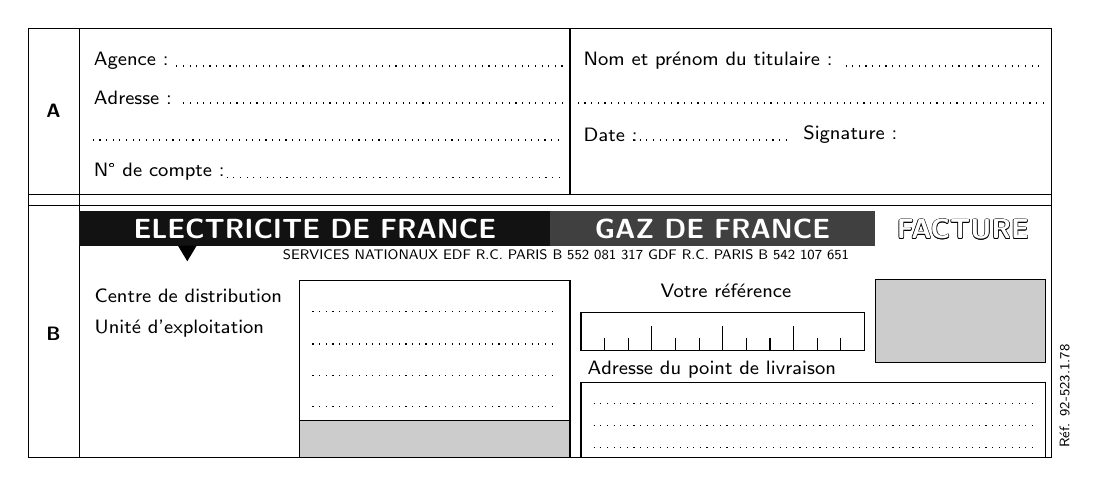
\begin{tikzpicture}[x=1cm,y=1cm,font=\sffamily\scriptsize]
\draw (0,0) rectangle (13,5.45);
\draw (.65,0)--(.65,5.45) (0,3.34)--(13,3.34) (0,3.20)--(13,3.20)
 (6.88,3.34)--(6.88,5.45);
\node at (.32,4.4) {\textbf{A}};
\node[anchor=west] at (.71,5.04) {Agence :}; \draw[dotted] (1.88,4.97)--(6.79,4.97);
\node[anchor=west] at (.71,4.57) {Adresse :}; \draw[dotted] (1.97,4.50)--(6.79,4.50);
\draw[dotted] (.82,4.03)--(6.79,4.03);
\node[anchor=west] at (.71,3.63) {N° de compte :}; \draw[dotted] (2.52,3.55)--(6.79,3.55);
\node[anchor=west] at (6.93,5.04) {Nom et prénom du titulaire :};
\draw[dotted] (10.38,4.97)--(12.89,4.97) (6.98,4.50)--(12.91,4.50);
\node[anchor=west] at (6.93,4.10) {Date :};
\draw[dotted] (7.68,4.03)--(9.69,4.03);
\node[anchor=west] at (9.72,4.10) {Signature :};
\node at (.32,1.57) {\textbf{B}};
\fill[black!93] (.65,2.69) rectangle (6.63,3.13);
\fill[black!75] (6.63,2.69) rectangle (10.75,3.13);
\node[text=white,font=\sffamily\bfseries] at (3.64,2.90) {ELECTRICITE DE FRANCE};
\node[text=white,font=\sffamily\bfseries] at (8.69,2.90) {GAZ DE FRANCE};
\foreach \dx/\dy/\ink in {-.22/0/black,-.16/.16/black,0/.22/black,.16/.16/black,.22/0/black,.16/-.16/black,0/-.22/black,-.16/-.16/black,0/0/white}{
  \node[xshift=\dx pt,yshift=\dy pt,text=\ink,font=\sffamily\bfseries] at (11.87,2.90) {FACTURE};
}
\fill (1.90,2.69)--(2.02,2.49)--(2.14,2.69)--cycle;
\node[font=\sffamily\tiny] at (6.83,2.57) {SERVICES NATIONAUX EDF R.C. PARIS B 552 081 317 GDF R.C. PARIS B 542 107 651};
\node[anchor=west] at (.72,2.05) {Centre de distribution};
\node[anchor=west] at (.72,1.63) {Unité d'exploitation};
\fill[black!20] (3.45,0) rectangle (6.88,.47);
\draw (3.45,0) rectangle (6.88,2.25) (3.45,.47)--(6.88,.47);
\foreach \y in {1.85,1.44,1.04,.65}{\draw[dotted] (3.61,\y)--(6.72,\y);}
\node at (8.86,2.11) {Votre référence};
\draw (7.02,1.36) rectangle (10.62,1.84);
\foreach \x in {7.32,7.62,8.22,8.52,9.12,9.42,10.02,10.32}{\draw (\x,1.36)--(\x,1.51);}
\foreach \x in {7.92,8.82,9.72}{\draw (\x,1.36)--(\x,1.67);}
\filldraw[fill=black!20] (10.76,1.20) rectangle (12.92,2.26);
\node[anchor=west] at (6.98,1.11) {Adresse du point de livraison};
\draw (7.02,0) rectangle (12.92,.95);
\foreach \y in {.68,.40,.12}{\draw[dotted] (7.18,\y)--(12.80,\y);}
\node[rotate=90,anchor=west,font=\sffamily\tiny] at (13.16,.00) {Réf. 92-523.1.78};
\end{tikzpicture}}}

En cas de désaccord sur le montant d'un prélèvement, je réglerai le différend directement avec EDF-GDF.

Il est entendu qu'aucun avis particulier ne me sera adressé lors de l'exécution, ou, éventuellement, de la non-exécution des prélèvements.

\begin{flushright}\small 3420\\\end{flushright}
\figure{\makebox[\linewidth][r]{
\begin{tikzpicture}[x=.19cm,y=.19cm]
\draw[line width=1.4pt] (.61,.75) .. controls (.46,.98) and (.10,.81) .. (.21,.57)
 .. controls (.30,.35) and (.48,.76) .. (.56,.43)
 .. controls (.62,.22) and (.33,.07) .. (.18,.27);
\draw (-.52,.04)--(.97,.04);
\node[anchor=north,font=\tiny] at (.36,.02) {\unsure{Sodel|Sodé}};
\end{tikzpicture}}}
% archive sheet number: 8
\scanpage{10}

1) $X$ espace topologique, $U,V$ ouverts, \unsure{conditions} \unsure{équivalentes}
\[
\begin{aligned}
\text{a)}\quad & U=\complement\overline V,\quad V=\complement\overline U\\
\text{b)}\quad & U\cap V=\varnothing,\quad\complement(U\cup V)\subset\overline U\cap\overline V
 \qquad\text{(d'où égalité.)}\\
\text{c)}\quad & U\cap V=\varnothing,\quad X=\overline{U\cup V},\quad\dot U=\dot V\\
\text{d)}\quad & \overline U\cap\overline V=\dot U=\dot V\ \unsure{\Leftarrow|?}
\end{aligned}
\]

$U$ et $V$ se déterminent \unsure{mutuellemt|mutuellem$^{\mathrm t}$}. Pour $U$ fixé, il existe $V$ ayant les propriétés \unsure{précédentes|précitées} \unsure{ssi} $V=\complement\overline U$ est dense dans $\complement U$.

\unsure{2|3}) $X$ espace topologique, $K\subset X$ fermé, $U_K^{\deleted{\unsure{\prime|3}}}$ et $\deleted{\unsure{V}}U'_K$ deux ouverts relatifs de $X$ tels que
\[
\resizebox{.99\linewidth}{!}{$\displaystyle
\overline U_K^{\deleted{\unsure{\prime|-}}}=K\smallsetminus U'_K,\quad
\overline{U'_K}=K\smallsetminus U_K,\quad
C=\overline U_K\cap\overline{U'_K}=
\underset{\deleted{\overline U_K\smallsetminus U_K\unsure{=}\overline{U'_K}\smallsetminus U^{\unsure{\prime}}_K}}
 {\overset{\inserted{\overline U_K\smallsetminus U_K=\overline{U'_K}\smallsetminus U'_K}}
 {\text{frontière commune}}}$}
\]
de $U_K$ et $U'_K$ \uline{dans $K$} \inserted{(fermé dans $X$)}. Soit $B=U_K\cap\dot K$, \deleted{donc} donc $B$ ouvert ds $\dot K$ et fermé ds $U_K$ donc \unsure{rel$^{\mathrm t}$.} fermé ds $X$, Alors on a, \unsure{posant} \inserted{\unsure{si} $B\cap C=\varnothing$.}
\[
\resizebox{\linewidth}{!}{$\displaystyle\left\{\begin{aligned}
&U=U_K\smallsetminus\deleted{\unsure{D}}B_{\deleted{\unsure{K}}}=\operatorname{Int}(U_K)\\
&V=X\smallsetminus\overline U_K^{\deleted{\prime}}=
 (\underbrace{X\smallsetminus U_K}_{\inserted{X_1}})\smallsetminus C=\operatorname{Int}(X_1)\\
&U=\complement\overline V,\ V=\complement\overline U,\qquad
 \dot U=\dot V=\overline U\cap\overline V=\complement(U\cup V)=B\cup C\\
&\deleted{U\cap K=U\subset K,\ V\cap K=V_K}\quad
 \underbrace{V\subset X_1}_{\inserted{\text{\unsure{diff.} }C}}
 \underbrace{{}\subset\overline V}_{\inserted{\text{diff }B}}
\end{aligned}\right.$}
\]

\uline{Cor} \deleted{Si $B\cap C=\varnothing$ i.e. $U_K\smallsetminus U$, Supposons} \inserted{Pour \unsure{que}} \deleted{$B$} $X_1=\complement U_K$ soit \unsure{loc} fermé, il \unsure{f. et s.} que $B=U_K\cap\dot K$ soit \deleted{fermé dans $X$, \unsure{alors}} \deleted{\unsure{dans} $B\cup$} \deleted{$B$ est ouvert et} fermé dans $\unsure{X_1|X}$, ou encore que ce soit un \unsure{sous-ensemble} \unsure{topologique} \deleted{dans $\dot K$, \unsure{et} posant $K=B'\amalg B$} \deleted{\unsure{de|sur} $\dot K$. Posant alors $\dot K=B'\amalg \unsure{B|B'}$} ou encore qu'il soit fermé ds $B\cup C$, ou encore que $\overline B\cap C=\varnothing$. [Il suffit pour ceci que $\dot K\cap C=\varnothing$ i.e. que $U_K\unsure{\cup|\amalg}V_K\supset K^{\unsure{\bullet|\cdot}}$]. \deleted{i.e. $U_K$ et $V_K$ sont}
% archive sheet number: 9
